\appendix

\section{Experimental details and extraction ablations}
\label{sec:details}

\paragraph{Training.} We set free bits to 0 rather than DreamerV3's reference default of 1.0. The
measured KL divergence settles near 1.8 nats, well above collapse, so the floor is inactive here. All
three trained models pass the acceptance checks; none were discarded.

\paragraph{Data split.} Training uses trajectories 0--203 of the 256-trajectory dataset. The
remaining 52 form the analysis set. We fit $C$ on those 52 trajectories and evaluate the
Section~\ref{sec:intervention} correction on the same 52, so the absolute effect is in-sample with
respect to invariant fitting. The recovered and random-constraint arms use the same trajectories.

\paragraph{Scoring the correction over a grid.} We score the slope of rollout error over the fixed
$\alpha$ grid rather than the minimum on that grid. Taking the minimum selects the most favourable of
five points after seeing the curve. In one diagnostic run that rule would have reported a 5.9\%
improvement for an arm whose error rose monotonically to twice baseline.

\paragraph{Flow alignment contributes reproducibility.} Holding the candidate family, data,
dimension, degree, and $\alpha$ grid fixed, we select $C$ either by the invariance criterion alone or
by the joint criterion. Conservation alone recovers energy at $0.950$ against $0.973$ for the joint
rule, and gives a slightly better mean intervention slope ($-0.087$ against $-0.077$, winning on two
of three models). The difference is in spread: recovery varies by $0.035$ across seeds under
conservation alone and by $0.008$ under the joint rule.

\paragraph{The pairing residual does not track recovery.} As the extraction dimension rises from 6 to
12, energy recovery improves from $0.721$ to $0.967$ while the pairing residual worsens from $0.738$
to $0.876$. Recovery already reaches $0.967$ at dimension 8, where the residual is lower at $0.813$.
The added dimensions do not carry energy while resisting the Hamiltonian fit: directions 7--12
account for 44.9\% of the residual and 43.5\% of the flow. Figure~\ref{fig:ldsweep} gives the sweep.

\section{Latent sensitivity analyses}
\label{sec:sensitivity}

For each direction $u$ of the extracted subspace we measure its variance and the damage a
displacement along it does to an imagination rollout,
\begin{equation}
V(u) = \operatorname{Var}(u^\top z), \qquad
D_H(u) = \mathbb{E}\bigl[L_H(z+\epsilon u) - L_H(z)\bigr],
\label{eq:leverage}
\end{equation}
with $L_H$ the $H$-step imagination error against the analysis set.

\paragraph{Calibrating the displacement.} At $\epsilon = 0.05|z|$ the damage is about $-0.5\%$ of
baseline with the sign varying across directions. Imagination is deterministic, so repeated
unperturbed rollouts are identical and these values are not sampling noise. Damage for the leading
direction runs $-0.5\%$, $+3.1\%$, $+18.1\%$, $+46.4\%$, and $+128.8\%$ at $\epsilon/|z|$ of $0.05$,
$0.10$, $0.25$, $0.50$, and $1.00$. We use $\epsilon = 0.25|z|$, the smallest displacement whose
damage exceeds 10\% of baseline while the response still grows smoothly.

A displacement does not decay under imagination. After 40 steps it retains $6.3\times$ its initial
size at $\epsilon = 0.05|z|$, $2.8\times$ at $0.25|z|$, and $1.9\times$ at $0.5|z|$, as medians over
the three models.

\paragraph{Variance and sensitivity at different horizons.} At a 40-step horizon the two rankings
anticorrelate on all three models ($-0.364$, $-0.259$, $-0.406$), with damage spanning
$13.5\times$ to $118.8\times$ between the most and least consequential direction
(Figure~\ref{fig:leverage}a). The ranking replicates: split-half rank correlation of $D_H$ has median
$0.95$ across the settings we tried, with a minimum of $0.52$ at the smallest displacement and
longest horizon. The disagreement with variance does not extend to long horizons. Pooling three
models and three displacements, median $\rho(V, D_H)$ is $-0.252$ at horizon 20, negative in 9 of 9
settings; $-0.196$ at horizon 50, negative in 5 of 9; and $-0.028$ at horizon 100, negative in 5 of
9, with one setting reaching $+0.727$. Once a rollout has diverged, high-amplitude directions
dominate the error and the rankings realign.

The correction pushes along higher-damage directions at $+0.385$, $+0.692$, and $+0.287$
(Figure~\ref{fig:leverage}b), without having been given that ranking. The correlations stay well
below $1$, so the correction is only partly concentrated there. All of this is measured on the
conservative models.

\begin{figure}[h]
\centering
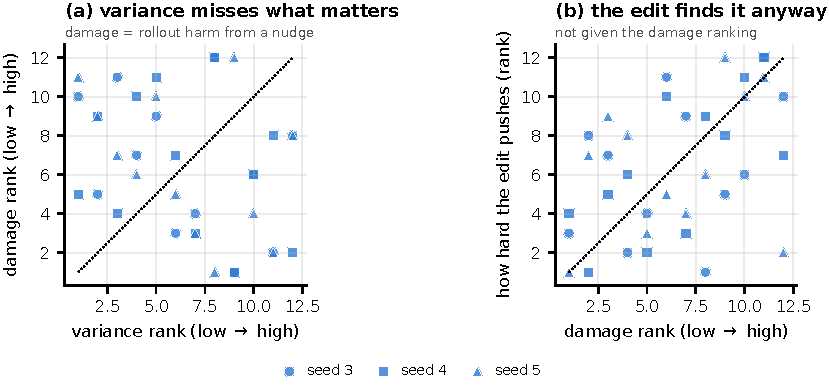
\includegraphics[width=\textwidth]{figures/fig4_leverage.pdf}
\caption{Each point is one of the 12 extracted directions, ranked within its own model; the dotted
line marks equal ranks. \textbf{(a)} Variance rank against damage rank at a 40-step horizon.
\textbf{(b)} Damage rank against the magnitude of the invariant correction along that direction.}
\label{fig:leverage}
\end{figure}

\paragraph{Basis-independent properties reproduce better than coordinate selectors.} The three models
agree closely on quantities that need no choice of basis: energy recovery varies by $0.008$,
intervention slopes by $0.016$, and the top-3 eigenvalue mass of
$M_C = \mathbb{E}[gg^\top/\|g\|^2]$ with $g = \nabla C$ by $0.046$ ($0.448$, $0.441$, $0.487$).
Selectors on individual coordinates are less stable: ranking coordinates by $\nabla C$ and keeping
the top three gives intervention slopes of $-0.075$, $+0.016$, and $-0.089$, beating a variance
ranking on two models and changing sign across seeds. An orthogonal projector onto the top eigenspace
of $M_C$ beats the variance selector on all three models, though on one it sits at the 41st
percentile of 100 random rank-3 subspaces. Since the correction is rank one at each state, the
spectrum of $M_C$ measures how much $\nabla C$ rotates as the state changes, and the amount is
similar across models. This is consistent with the models encoding the same scalar in different
latent coordinate systems, although we do not directly align their representations.

\section{Additional sweeps}
\label{sec:sweeps}

\paragraph{Energy outside the highest-variance directions.} On two of three models, principal
directions 7--12 carry about twice the energy information of the top six ($2.23\times$ and
$2.13\times$); on the third the ratio reverses to $0.91$. We report the models separately because a
median would hide the sign change. Figure~\ref{fig:lowvar} shows the decomposition.

\paragraph{Accumulated invariant error.} Accumulated invariant error predicts which rollouts degrade
most: an integral predictor reaches $R^2 = 0.187$ against $0.021$ for a fitted power law in time at
the horizon where both perform best, and shuffling destroys the relation. The current experiments do
not distinguish weighted from unweighted accumulation. In a nested comparison with 400 bootstrap
resamples, the weighted term adds explanatory power beyond the unweighted term in 1 of 9
seed--horizon combinations, and the unweighted beyond the weighted in 0 of 9, at $n = 512$.

\begin{figure}[h]
\centering
\begin{minipage}[t]{0.36\textwidth}
\centering

\includegraphics[width=\textwidth]{figures/fig2_ld_sweep.pdf}
\caption{Energy recovery and pairing residual against extraction dimension. Lines are medians over
the three models; points are individual models. Both quantities are dimensionless.}
\label{fig:ldsweep}
\end{minipage}\hfill
\begin{minipage}[t]{0.58\textwidth}
\centering

\includegraphics[width=\textwidth]{figures/fig3_low_variance.pdf}
\caption{\textbf{(a)} Energy-probe $R^2$ for the top six principal directions against directions
7--12, per model. \textbf{(b)} Fraction of latent flow and pairing residual carried by each group,
medians over three models.}
\label{fig:lowvar}
\end{minipage}
\end{figure}
